\documentclass{article}
\usepackage{122}

\usepackage{graphicx}
\usepackage{epsdice}

\newcommand{\hr}{\par\vspace{.5\baselineskip}\noindent\hrulefill\par}

\title{Теория вероятности \\ ДЗ семинара №3}

\begin{document}
  \maketitle

  \hr
  \section*{Домашнее задание}
  \section*{№19}
  $\ds P(B|A) = P(5 + \epsdice{4} = 9) = \f{1}{6} $ \\
  $\ds P(B) = P(\epsdice{4}\,\epsdice{5}) + P(\epsdice{5}\,\epsdice{4}) + P(\epsdice{3}\,\epsdice{6}) + P(\epsdice{6}\,\epsdice{3})
  = \f{4}{36} = \f{1}{9} $ \\
  вот поэтому они ненезависимые

  \section*{№20}
  $P(AB)$ всегда $\leq \min\l(P(A),\, P(B)\r)$ \\
  тоесть у нас $\ds P(AB) \leq \f{1}{3}$ \\
  получается выражение $\ds P(AB) \leq \f{3}{8}$ теоретически верно тк $\ds \f{3}{8} > \f{1}{3}$

  \section*{№22}
  $\ds P(n) = 1-\l(1-0.01\r)^n$ \\
  $\ds P(x) = 1-\l(1-0.01\r)^x \geq 0.95$ \\
  $\ds 0.05 \geq 0.99^x $ \\
  $\ds \ln\l(0.05\r) \geq \ln\l(0.99^x\r) $ \\
  $\ds \ln\l(0.05\r) \geq x\ln\l(0.99\r) $ \\
  $\ds \f{\ln\l(0.05\r)}{\ln\l(0.99\r)} \leq x $ \\
  $\ds 298.07285221322263 \leq x $ \\
  $\ds x \geq 299 $

  \section*{№36}
  $\ds P(n) = \l(\f{1}{2}\r)^n$ \\
  тоесть ответ у нас один

  \section*{№37}
  карты пик всегда чёрные, и поэтому $P(B|A) = 0$ и они ненезависимые

  \section*{№40}
  $\ds P(A) = p_1 \cdot \l(1 - \l(1 - p_2\r)\cdot\l(1 - p_3\r)\r) = 0.704$

  \section*{№43}
  $\ds P(A) = 1 - \l(1 - p_4\r)\cdot\l(1 - p_3 \cdot \l(1 - \l(1 - p_1\r)\cdot\l(1 - p_2\r)\r)\r) = 0.782$ \\
  $\ds P(A) = p_6 \cdot \l(1 - \l(1 - p_2\r)\cdot\l(1 - p_1\r)\r) \cdot \l(1 - \l(1 - p_5\r)\cdot\l(1 - p_3\cdot p_4\r)\r) = 0.16356$

  \section*{№46}
  TODO

  \section*{№82}
  TODO

  \section*{№83}
  \begin{enumerate}[label=\realasbuk*)]
    \item $\ds P(A) = \f{C^3_4}{C^3_{10}} = \f{1}{30}$
    \item $\ds P(A) = 0.4^3 = 0.064$
  \end{enumerate}

  \hr
  \section*{Условия}
  \includegraphics[page=45, width=0.3\textwidth]{./books/учебник теорвер.pdf} \hfill
  \includegraphics[page=46, width=0.3\textwidth]{./books/учебник теорвер.pdf} \hfill
  \includegraphics[page=47, width=0.3\textwidth]{./books/учебник теорвер.pdf} \hfill

  \section*{Ответы}
  \begin{center}
    \includegraphics[page=214, width=0.7\textwidth, trim={0 0cm 0 7cm}, clip]{./books/учебник теорвер.pdf}
  \end{center}

\end{document}
